

\chapter[Restoration Efforts: The Kok-Aral Dam]{Restoration Efforts:\\The Kok-Aral Dam}
\label{cp:restoration}

\vspace{.935em}

In 2005, Kazakhstan constructed the Kok-Aral Dam across the Syr Darya River to address the dire state of the North Aral Sea (\autoref{fig:kok-aral-dam}). This project aimed to restore water levels, reduce salinity, and improve local ecosystems.  By retaining more water within the northern basin, the dam has improved water quality, supported the recovery of aquatic life, and promoted the reappearance of wetland habitats. While the South Aral Sea remains beyond recovery, the dam has brought significant benefits to the northern basin \autocite{chen2018kazakhstan}.

\section{Successes of the Kok-Aral Dam}
The primary achievement of the Kok-Aral Dam was the rise in water levels of the North Aral Sea, which increased by about 3 meters \autocite{chen2018kazakhstan}. This helped restore local ecosystems and reduce the salinity, which had previously risen to harmful levels. As a result, fish populations, including the native bream, pike-perch and roach, returned to the region, providing some revival for the fishing industry. Wetlands also reappeared, offering habitat for migratory birds that had previously abandoned the area \autocite{chen2018aral}.

\begin{figure}[htpb]
    \centering
    \fbox{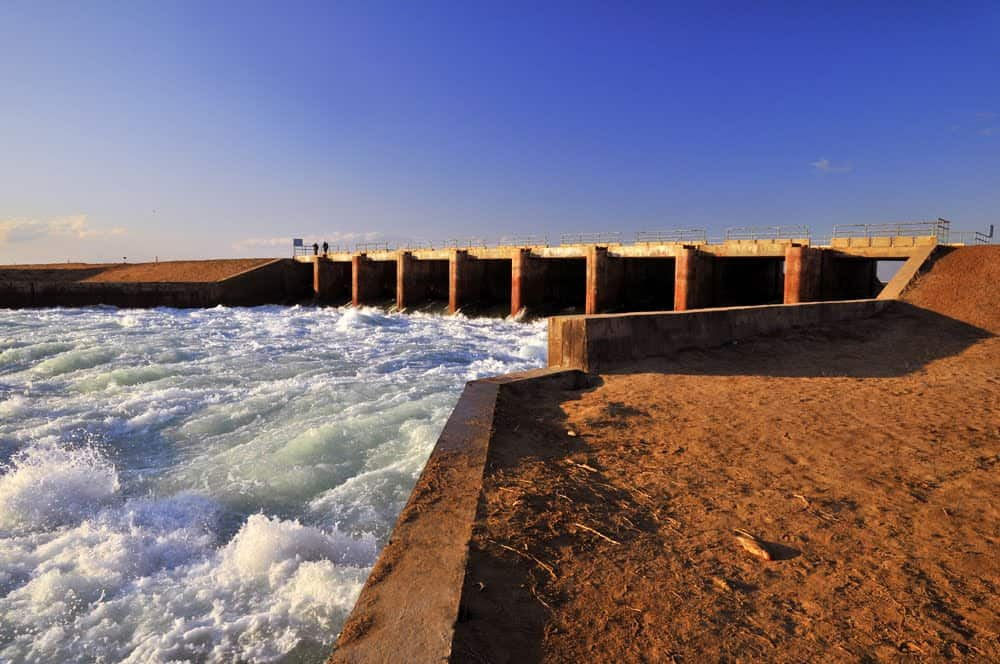
\includegraphics[width=0.7\linewidth]{Figures/Kok-Aral Dam.png}}
    \caption{Kok-Aral Dam}
    \label{fig:kok-aral-dam}
\end{figure}

\section{Challenges for the South Aral Sea}
Despite the successes in the North Aral Sea, the South Aral Sea remains largely beyond recovery. The southern basin continues to suffer from severe ecological degradation, with its waters having retreated significantly, leaving behind a toxic desert. The scale of this deterioration and the lack of resources for large-scale restoration mean that the South Aral Sea is unlikely to recover in the near future \autocite{chen2018aral}.

\section{The Way Forward}
The success of the Kok-Aral Dam underscores the potential of localized restoration efforts, but it also highlights the need for regional cooperation. While Kazakhstan has made progress, sustained recovery of the Aral Sea region will require collective action from all stakeholders to address inefficient water management and unsustainable agriculture, ultimately restoring ecological balance \autocite{dukhovny2003lessons}.